

\actTitle{Worksheet 1.8}



\noindent \textbf{Instructions:}  Work together in groups of  3 or 4 to complete the following problems.




\begin{enumerate}
\item Given $f(x)=5x^2+2x-3$ and $g(x)=x+3$.
\begin{enumerate}
\item Find $(f \circ g)(x)$.
\vfill


\item  Find $(g \circ f)(x)$.
\vfill
 
 \item Find $(f \circ g)(1)$.
 \vfill
 
 \item  Find $(g \circ f)(1)$.
 
 \vfill
 \end{enumerate}

\clearpage

\item Given $f(x)=x^2$ and $g(x)=\sqrt{x}$.
\begin{enumerate}
\item Determine the domains of $f(x)$ and $g(x)$.\vfill
\item Find $(f \circ g)(x)$ and simplify completely.\vfill
\item Determine the domain of $(f \circ g)(x)$.  Keep in mind that the domain of a function is the collection of $x$-values that can be plugged into the function.\vfill
\item  Find $(g \circ f)(x)$ and simplify completely.\vfill
\item Determine the domain of $(g \circ f)(x)$.\vfill
\item What do you notice about $(f \circ g)(x)$ and $(g \circ f)(x)$?  What do you notice about their domains?  Does the domain of the inside function affect the domain of function composition?\vfill
\end{enumerate}




\vfill

\clearpage 

\item Let $f(x)=x^2-1$, $g(x)$ be given by the graph below, and $h(x)$ be given by the table below.


\begin{minipage}[t]{.75\textwidth}
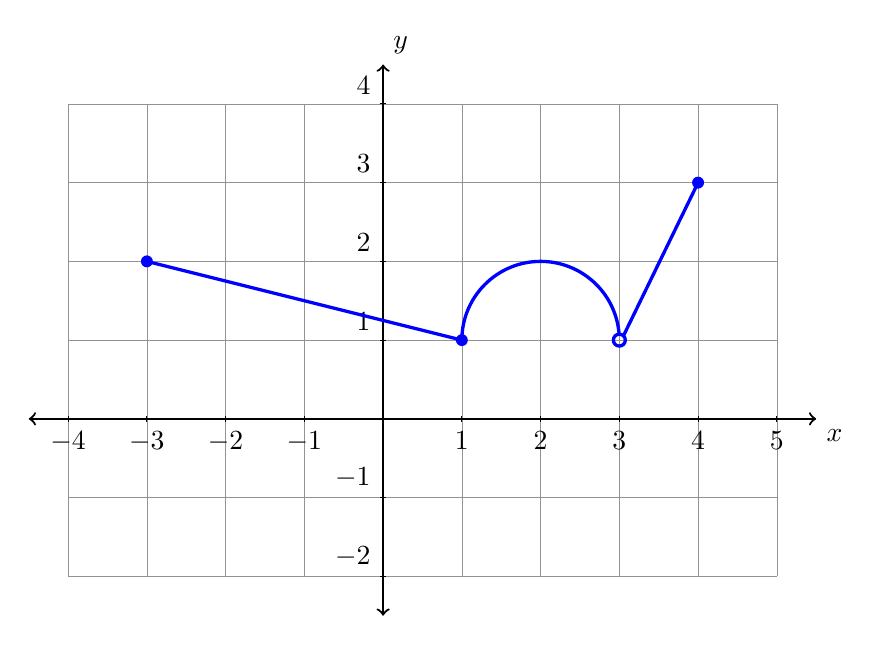
\begin{tikzpicture}[y=1cm, x=1cm,font=\sffamily,
	mydot/.style={
    circle,
    fill=white,
    draw,
    outer sep=0pt,
    inner sep=1.5pt
  }]
    %% Add a grid
    \draw[step = 1, gray, very thin,opacity=0.85] (-4, -2) grid (5, 4);
 	%% Draw the axes
	\draw[thick,<->] (-4.5,0) -- coordinate (x axis mid) (5.5,0) node[anchor = north west] {$x$};
    \draw[thick,<->] (0,-2.5) -- coordinate (y axis mid) (0,4.5) node[anchor = south west] {$y$};
    %% Label the y axis
    \foreach \y in {-2,...,-1,1,2,...,4} {
      \draw (1pt, \y) -- (-1pt, \y) node[anchor = south east] {$\y$};
    }
    %% Label the x axis
    \foreach \x in {-4,...,-1,1,2,...,5} {
      \draw (\x,1pt) -- (\x,-1pt) node[anchor = north] {$\x$};
    }
    %% Draw the function.
    \begin{scope}
         \draw[very thick,blue] (-3,2) -- (1,1);
         \draw[very thick,blue] (3.05,1.05) -- (4,3);
    %semi-circle
         \draw[very thick, blue] (1,1) arc [radius=1, start angle=180, end angle= 5];
     %parabola
     %    \draw[ultra thick, blue, domain=-5:0] plot (\x, {(-0.2)*(\x-5)*(\x+5)});
     %dots
         \fill[blue] (-3, 2) circle[radius=0.5ex];
         \fill[blue] (1,1) circle[radius=0.5ex];
         \fill[blue] (4,3) circle[radius=0.5ex];
         \draw[very thick, blue] (3,1) circle[radius=0.5ex];


    \end{scope}

    %%\node[above=0.1cm] at (-2,2 )   {\nextXValue};

  \end{tikzpicture}
\end{minipage}
%second column
\begin{minipage}[t]{.25\textwidth}
\vspace{-2in}
\begin{tabular}{|l|l|}
\hline
\textbf{$x$} & \textbf{$h(x)$} \\ \hline
-3           & 2               \\ \hline
0            & 4               \\ \hline
1            & 5               \\ \hline
3            & -6              \\ \hline
\end{tabular}
\end{minipage}







\begin{enumerate}
\item Determine the $(f\circ g)(4)$.\vfill
\item Determine the $(g\circ h)(-3)$.\vfill
\item Determine the $(h\circ f)(1)$..\vfill
\item Determine the $(g\circ f)(2)$.\vfill
\end{enumerate}


\clearpage

\item Given $f(x)=4x-9$ and $g(x)=\sqrt{x+6}$
\begin{enumerate}
\item Find $\displaystyle\left(\frac{f}{g}\right)(x)$ and determine its domain.
\vfill
\item Find $\displaystyle\left(\frac{g}{f}\right)(x)$ and determine its domain.
\vfill
\end{enumerate}

\item Given $f(x)=2x^2-5x+1$.  Find the difference quotient, $\displaystyle \frac{f(x+h)-f(x)}{h}$.
\vfill
\vfill



\end{enumerate}




